%!TEX root = 1_power_supply.tex
\documentclass[1_power_supply.tex]{subfiles}
\graphicpath{{../figures}}
\begin{document}

\section{電源システムの評価}

  \subsection{目的}

    これまでの実験で使った回路を組み合わせて,電源システム全体としての特性を評価する.

  \subsection{方法}

    電源システム全体を図\ref{fig:4_power_supply}に示す.


    \begin{figure}[htbp]
      \begin{center}
        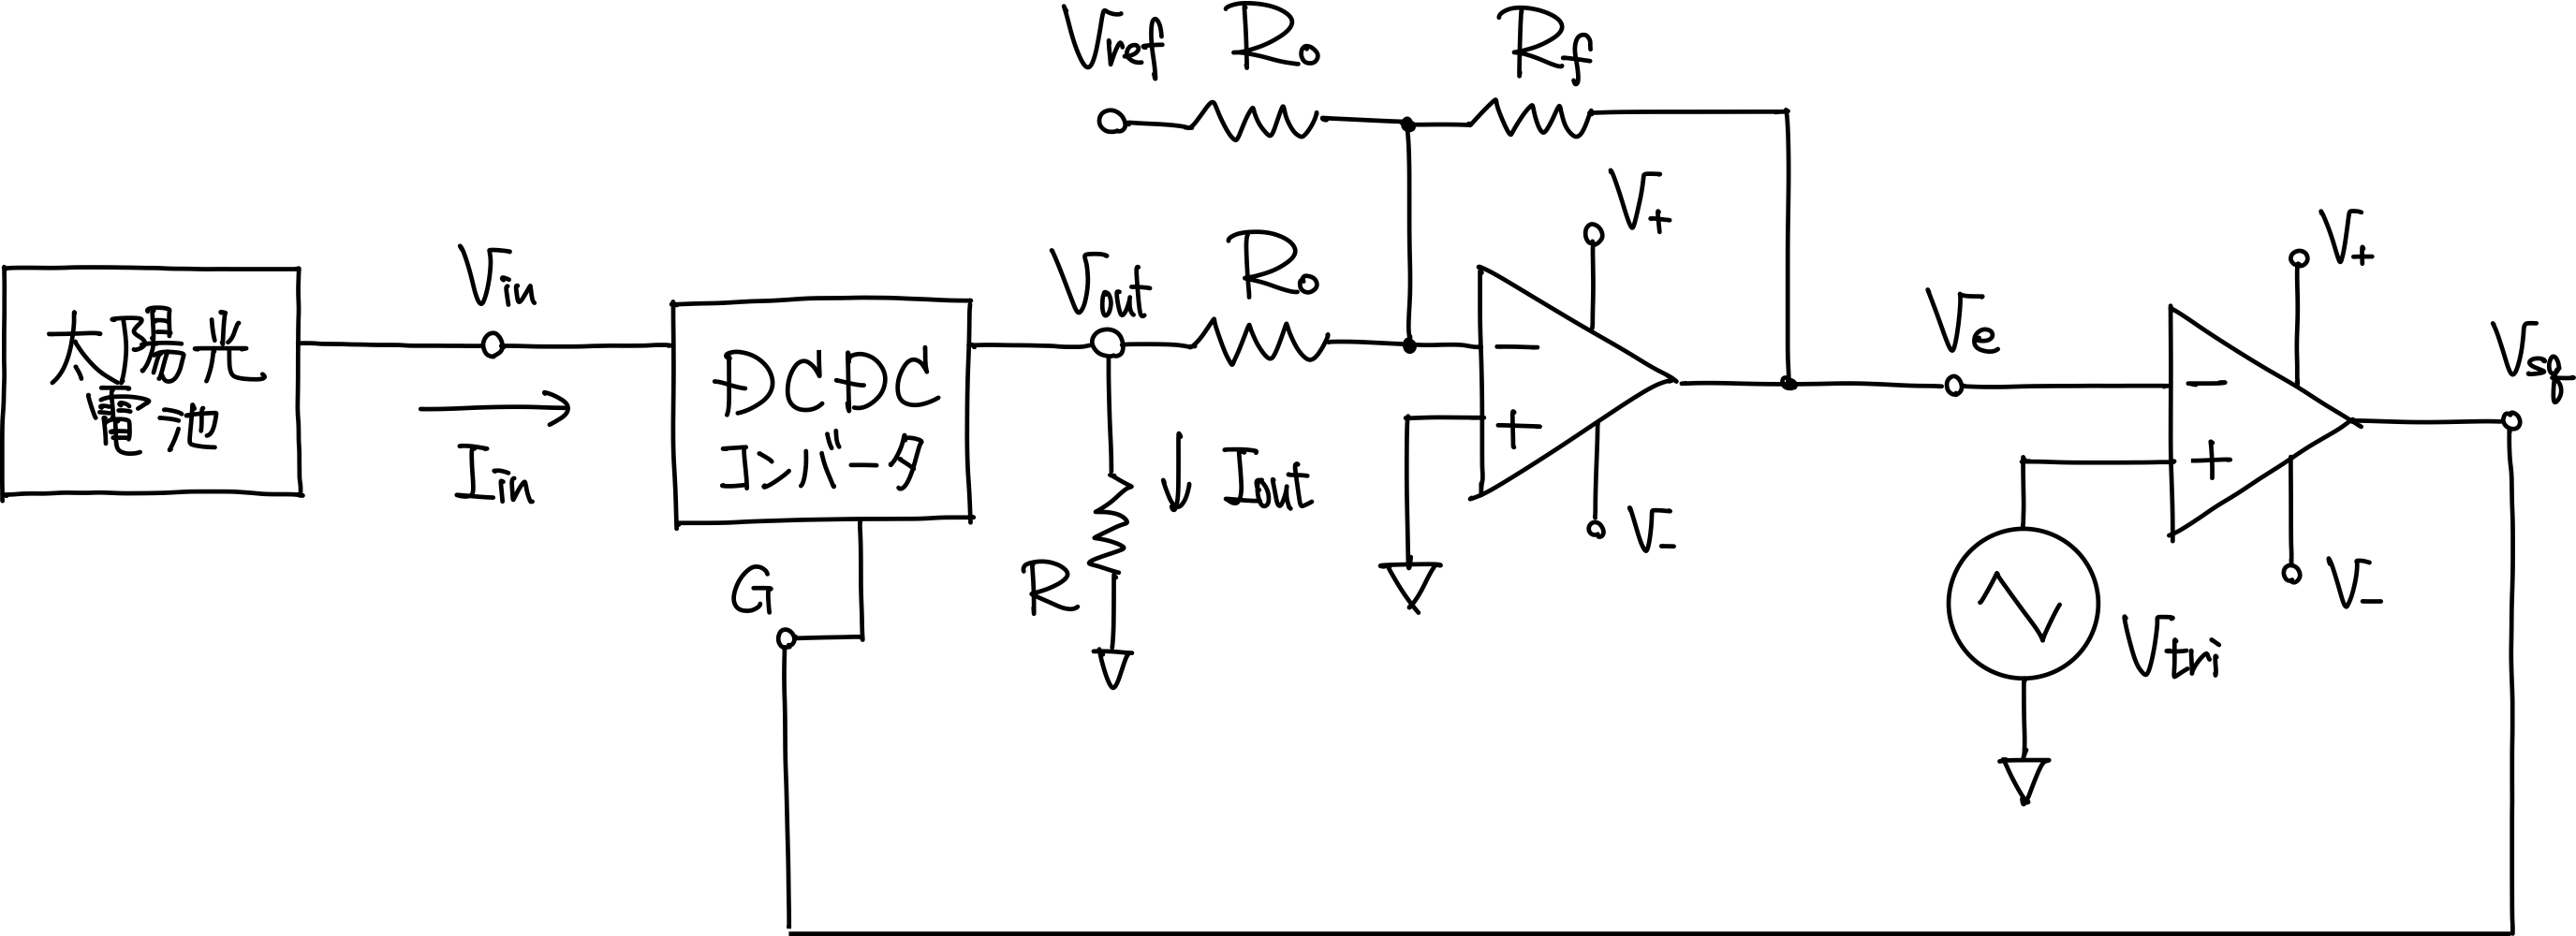
\includegraphics[width=0.8\columnwidth]{4_power_supply.png}
        \caption{電源システムの回路図}\label{fig:4_power_supply}
      \end{center}
    \end{figure}

    \begin{itemize}
      \item $R_0 = \SIs{2}{\kilo\ohm}$
      \item $R_\mathrm{f} = \SIs{10}{\kilo\ohm}$
      \item $V_\mathrm{tri} = \SIs{13}{\volt}$(peak-to-peak)
      \item (三角波の周波数) = $\SIs{50}{\kilo\hertz}$
      \item $V_+ = \SIs{15}{\volt}$
      \item $V_- = \SIs{-15}{\volt}$
    \end{itemize}
    と設定する.$R_0,R_\mathrm{f}$の値から分かるように,今回の測定では$K_\mathrm{fb}=-5$で固定とする.$\mathrm{AC}=\SIs{55.5}{\centi\meter},\SIs{85.5}{\centi\meter}$の場合で,$V_\mathrm{ref}$を変化させて入力電圧・電流,出力電圧・電流を測定する.

  \subsection{結果}

    目標電圧$V_\mathrm{ref}$と,入力電圧・電流,出力電圧・電流との関係を図\ref{fig:4_vin}-\ref{fig:4_iout}に示す.


    \begin{figure}[htbp]
      \centering
      \begin{minipage}{0.45\columnwidth}
        \centering
        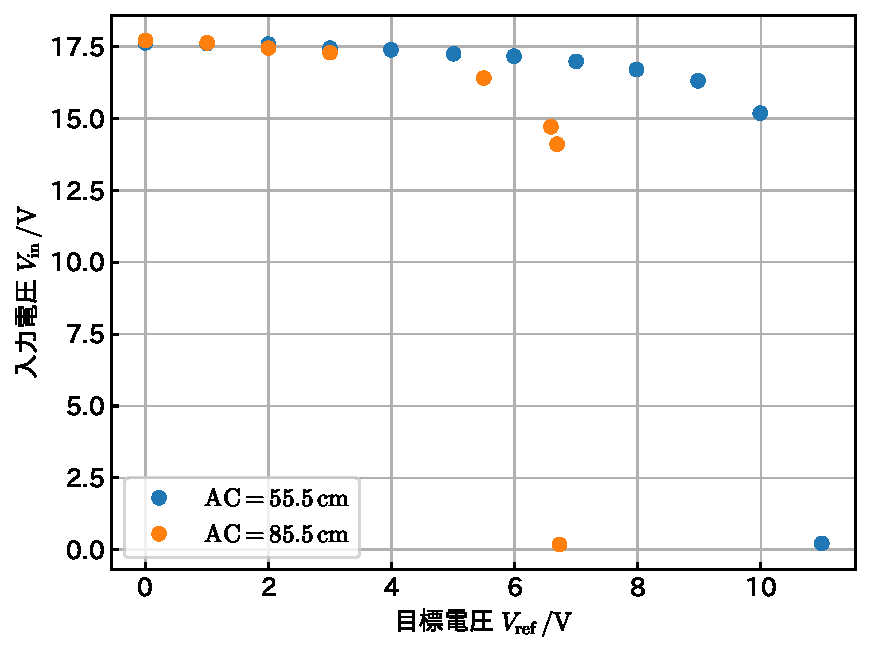
\includegraphics[width=0.8\columnwidth]{4_-5_vin.pdf}
        \subcaption{入力電圧}\label{fig:4_vin}
      \end{minipage}
      \begin{minipage}{0.45\columnwidth}
        \centering
        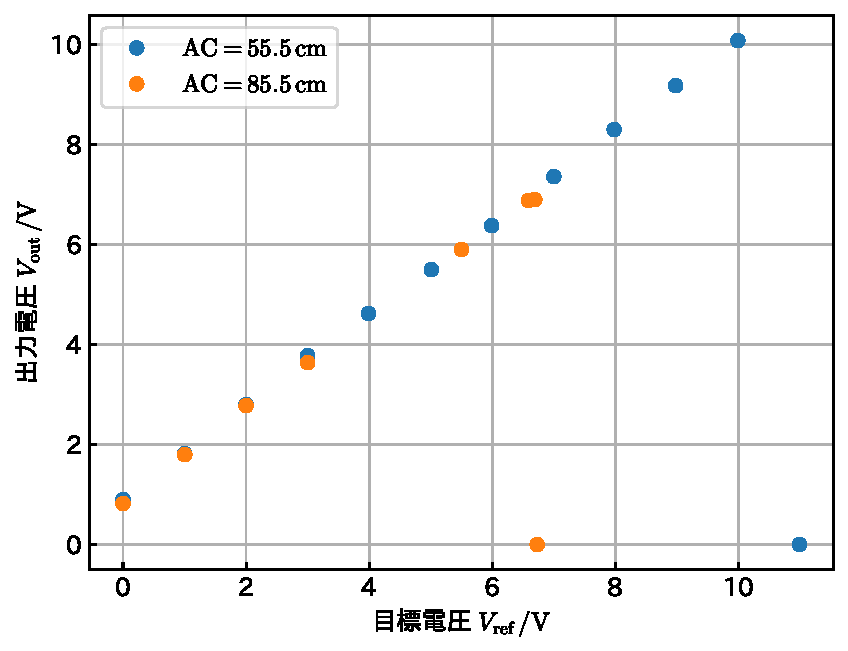
\includegraphics[width=0.8\columnwidth]{4_-5_vout.pdf}
        \subcaption{出力電圧}\label{fig:4_vout}
      \end{minipage}
      \hspace{5mm}
      \begin{minipage}{0.45\columnwidth}
        \centering
        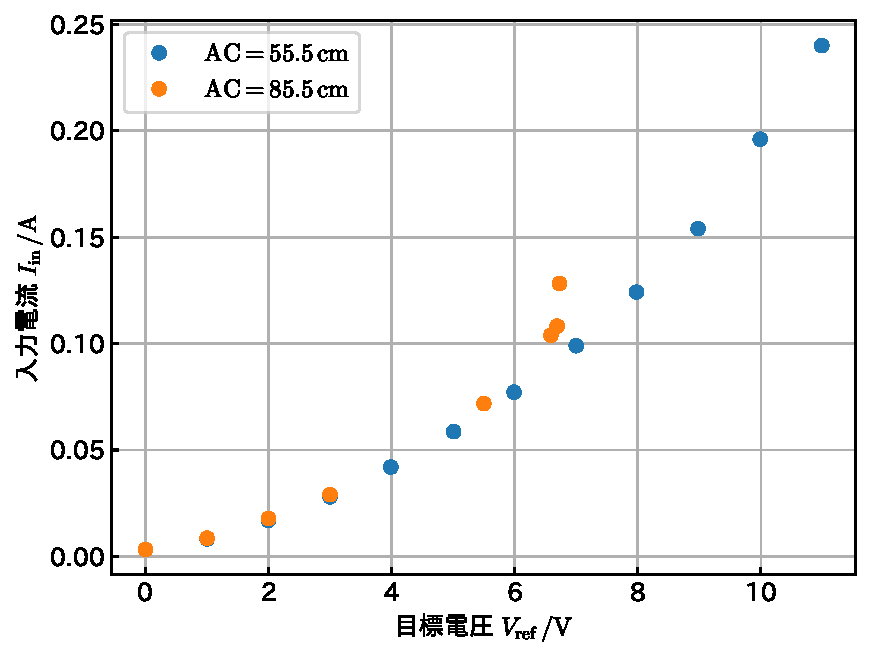
\includegraphics[width=0.8\columnwidth]{4_-5_iin.pdf}
        \subcaption{入力電流}\label{fig:4_iin}
      \end{minipage}
      \begin{minipage}{0.45\columnwidth}
        \centering
        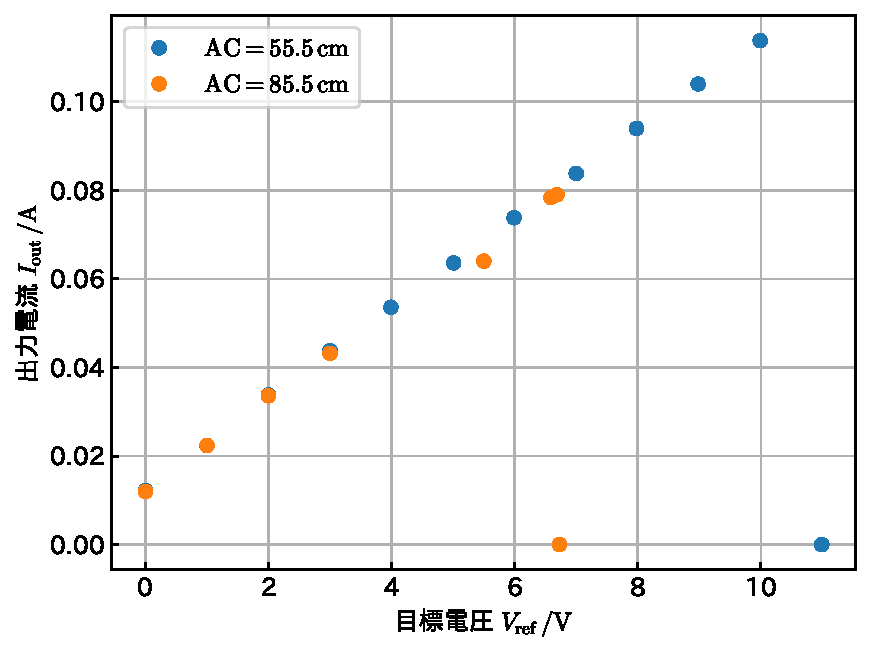
\includegraphics[width=0.8\columnwidth]{4_-5_iout.pdf}
        \subcaption{出力電流}\label{fig:4_iout}
      \end{minipage}
      \caption{各測定の結果}
      \label{figs:4_result}
    \end{figure}
    $\mathrm{AC}=\SIs{55.5}{\centi\meter}$のときは$V_\mathrm{ref}=\SIs{11}{\volt}$,$\mathrm{AC}=\SIs{85.5}{\centi\meter}$のときは$V_\mathrm{ref}=\SIs{6.7}{\volt}$で大きく測定値が変化していることがわかる.

  \subsection{考察}

    入力電流・電圧,出力電流・電圧からそれぞれ入力電力,出力電力を計算しプロットしたものをそれぞれ\ref{fig:4_pin},\ref{fig:4_pout}に,電力効率をプロットしたものを\ref{fig:4_eff}に示す.


    \begin{figure}[htbp]
      \centering
      \begin{minipage}{0.45\columnwidth}
        \centering
        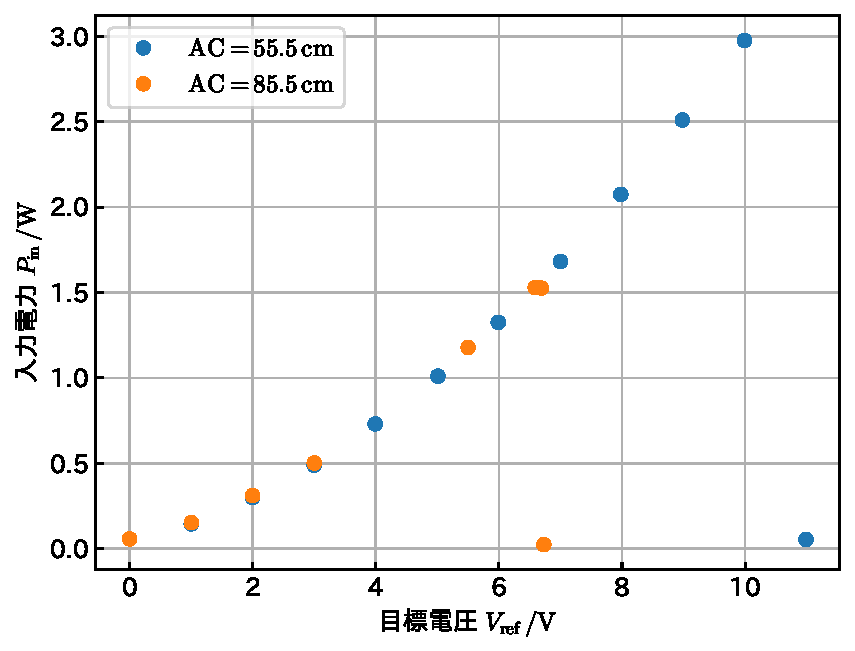
\includegraphics[width=0.8\columnwidth]{4_-5_pin.pdf}
        \subcaption{入力電力}\label{fig:4_pin}
      \end{minipage}
      \begin{minipage}{0.45\columnwidth}
        \centering
        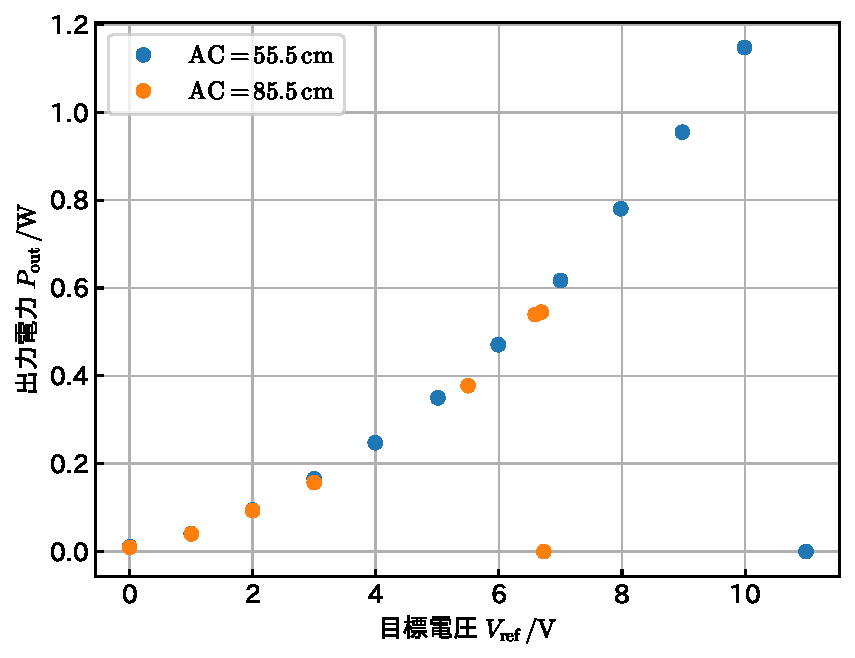
\includegraphics[width=0.8\columnwidth]{4_-5_pout.pdf}
        \subcaption{出力電力}\label{fig:4_pout}
      \end{minipage}
      \hspace{5mm}
      \begin{minipage}{\columnwidth}
        \centering
        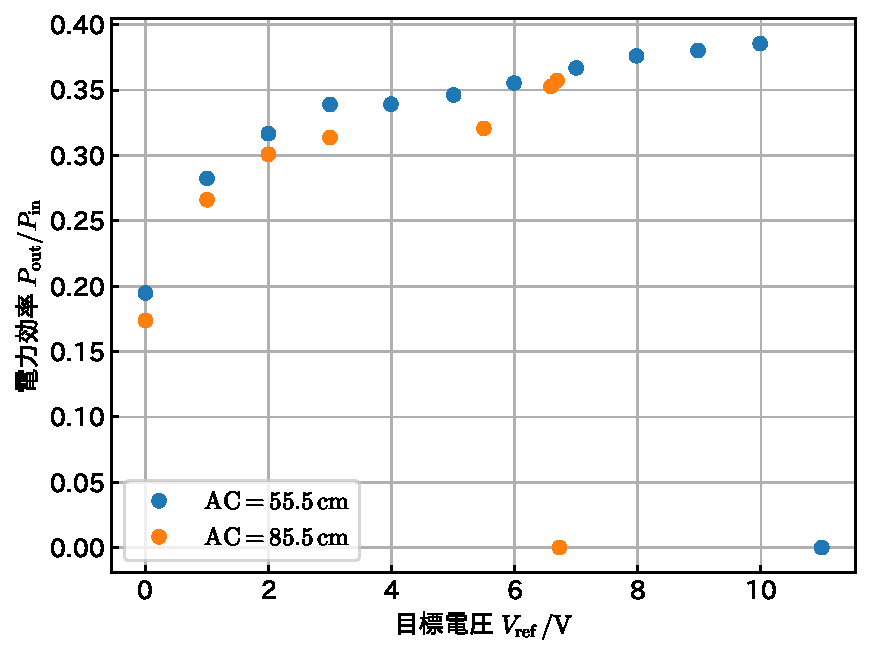
\includegraphics[width=0.8\columnwidth]{4_-5_eff.pdf}
        \subcaption{電力効率}\label{fig:4_eff}
      \end{minipage}
      \caption{電力のプロット}
      \label{figs:4_think}
    \end{figure}


    \begin{figure}[htbp]
      \begin{center}
        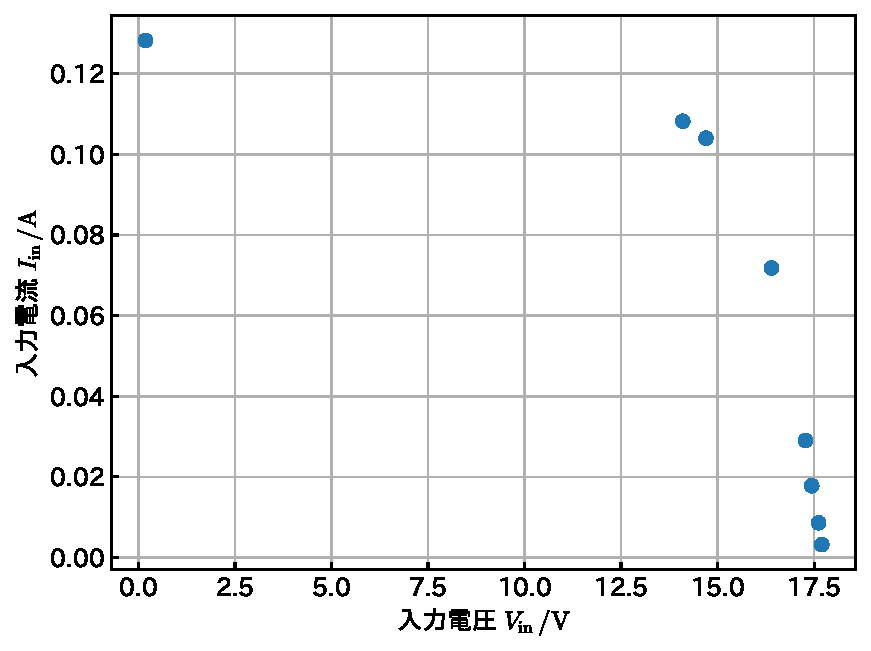
\includegraphics[width=0.8\columnwidth]{4_-5_90_vi.pdf}
        \caption{入力の電圧-電流特性($\mathrm{AC}=\SIs{85.5}{\centi\meter}$)}\label{fig:4_v-i}
      \end{center}
    \end{figure}

    電力効率は,目標電圧が0である点と測定点が大きく変化する点を除いて$\SIs{25}{\percent}\sim\SIs{40}{\percent}$となった.なお,入力の電流・電圧特性は図\ref{fig:4_v-i}に示すとおりで,$(V_\mathrm{in},I_\mathrm{in})=(\SIs{6.90}{\volt}, \SIs{0.0790}{\ampere})$のときに最大電力で動作することが分かる.

    また,測定点が大きく変化した(途切れた)点の原因については,差信号$V_\mathrm{e}$が三角波の振幅よりも大きくなり,デューティ比が1になったからと考える.

\end{document}
